

\subsection*{Problem 1.5}
\addcontentsline{toc}{subsection}{Problem 1.5}

The simulation of the attitude dynamics of the closed-loop system with control law given by \eqref{eq:control_law_attitude2} is in the file {\color{blue} attitude2.m}. For each time iteration,
the desired attitude $\mathbf{q}_d(t)$ given by $\phi(t) = 10\sin(0.1t), \theta(t) = 0, \psi(t) = 15\cos(0.05t)$, was converted to radians and then converted to quaternions by the use of the \texttt{MATLAB} function \texttt{euler2q()}. The desired quaternion value was then conjugated and cross multiplied with the current $\mathbf{q}$ iteration by the use of the \texttt{MATLAB} functions \texttt{quatconj()} and \texttt{quatmultiply()} respectively, as explained in equation \eqref{eq:q_product}. By doing so, $\mathbf{\tilde{q}}$ was calculated as per equation \eqref{eq:q_tilde}.

The $\tilde{\boldsymbol{\epsilon}}$ part of $\mathbf{\tilde{q}}$ was extracted and combined with $\boldsymbol{\omega}$ to create the state error and was multiplied with the $\mathbf{K}$ , equation \eqref{eq:K}, to create the control input in the same way as in {\color{blue} attitude1.m}. The initial values were kept the same as in exercise 1.3 and the $k_p$ and $k_d$ were changed to 10 and 300 respectively. 

\subsubsection*{Simulation results}
\addcontentsline{toc}{subsubsection}{Simulation results}

The simulation  of  {\color{blue} attitude2.m} resulted in the plots given in \Cref{fig:sim_attitude2_euler} and \Cref{fig:sim_attitude2_track}.

\begin{figure}[!htb]
	\centering
	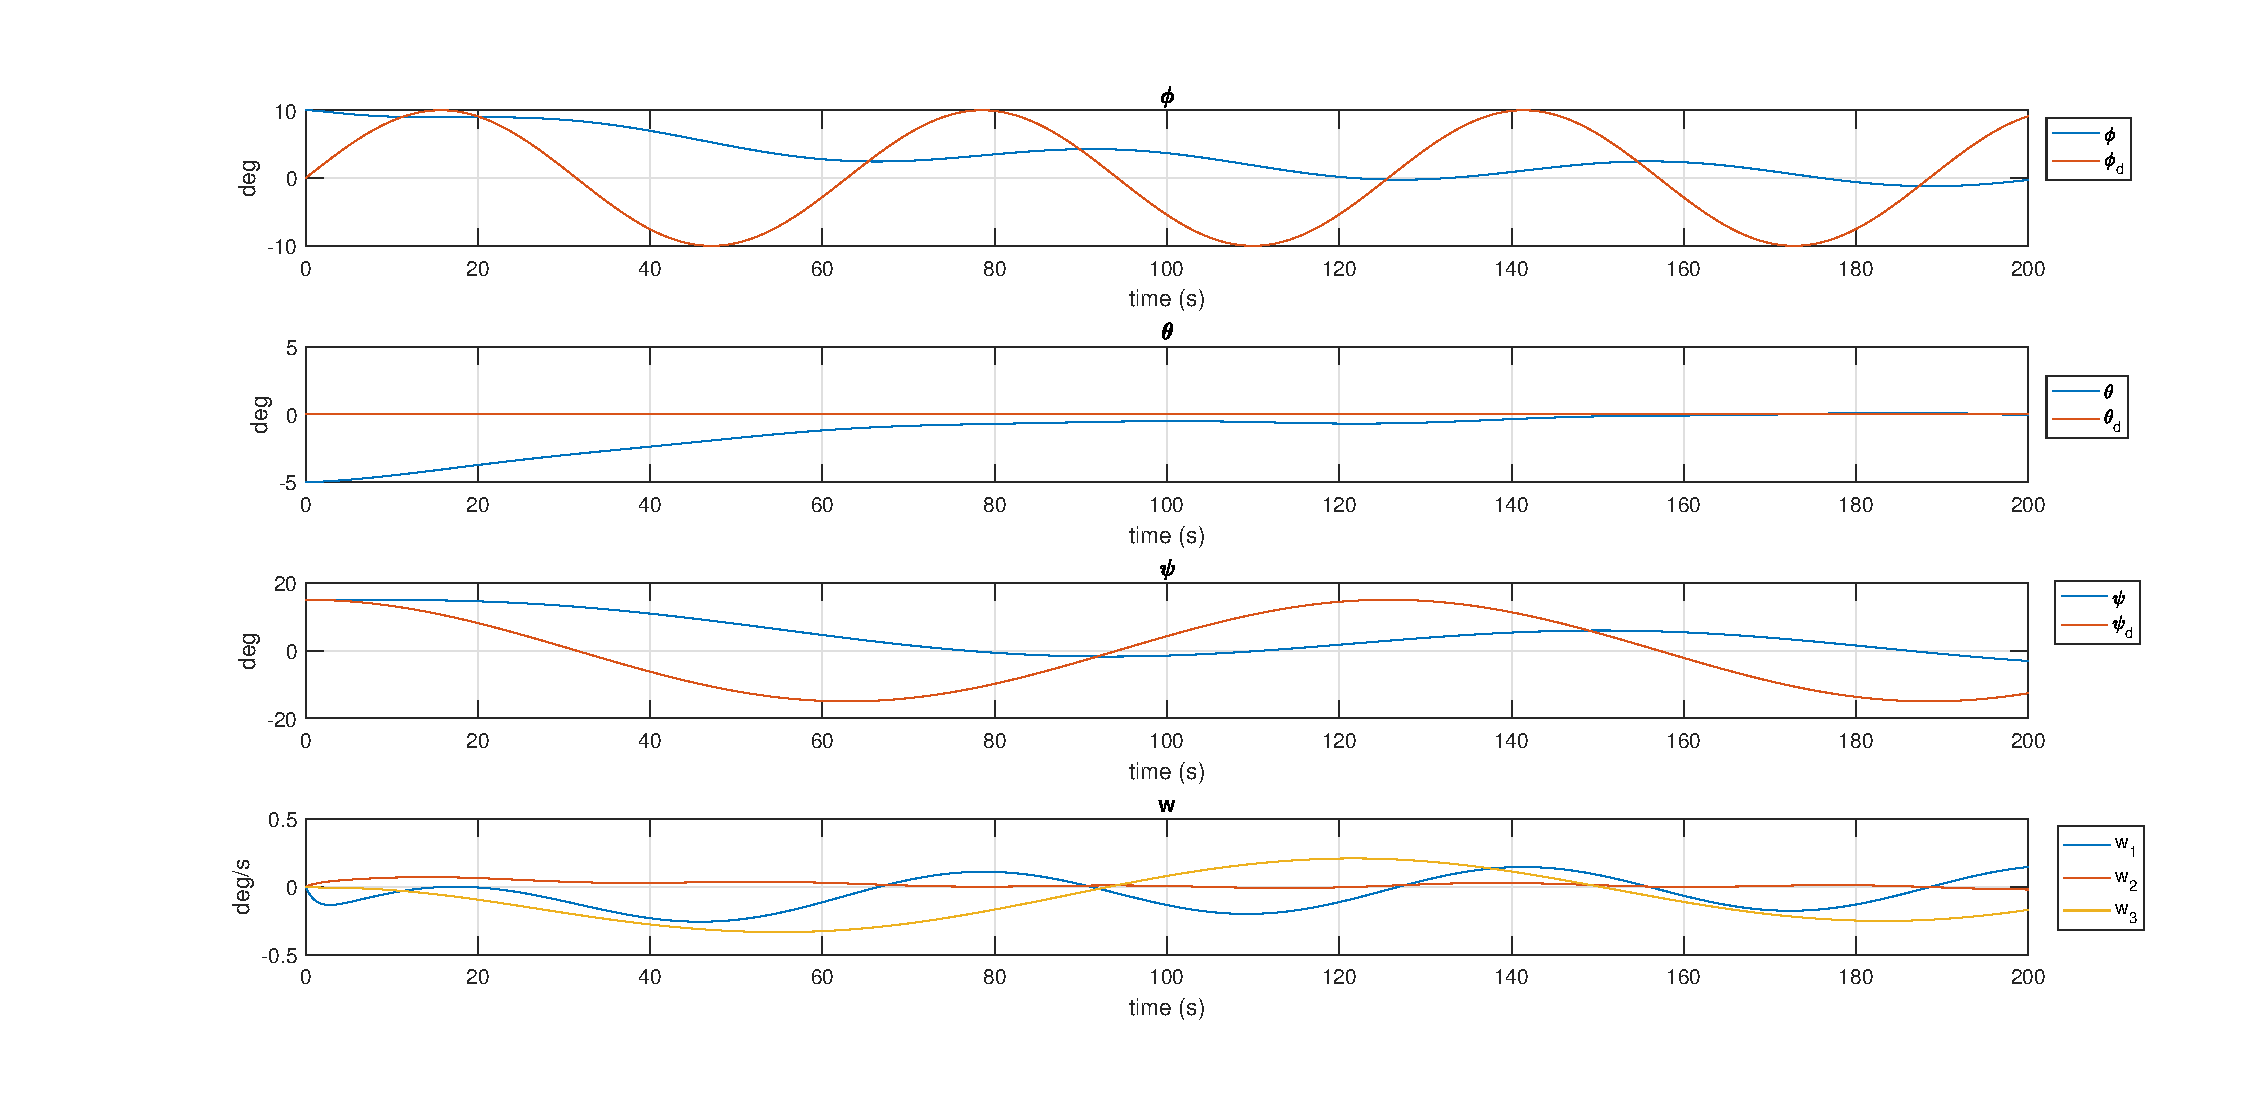
\includegraphics[width=1.00\textwidth]{figures/2_euler.eps}
	\caption{The resulting output euler angles with their corresponding desired values and the resulting output $\boldsymbol{\omega}$ (denoted $\mathbf{w}$ in the plot) from the simulation in attitude2.m.}
\label{fig:sim_attitude2_euler}
\end{figure}

\begin{figure}[!htb]
	\centering
	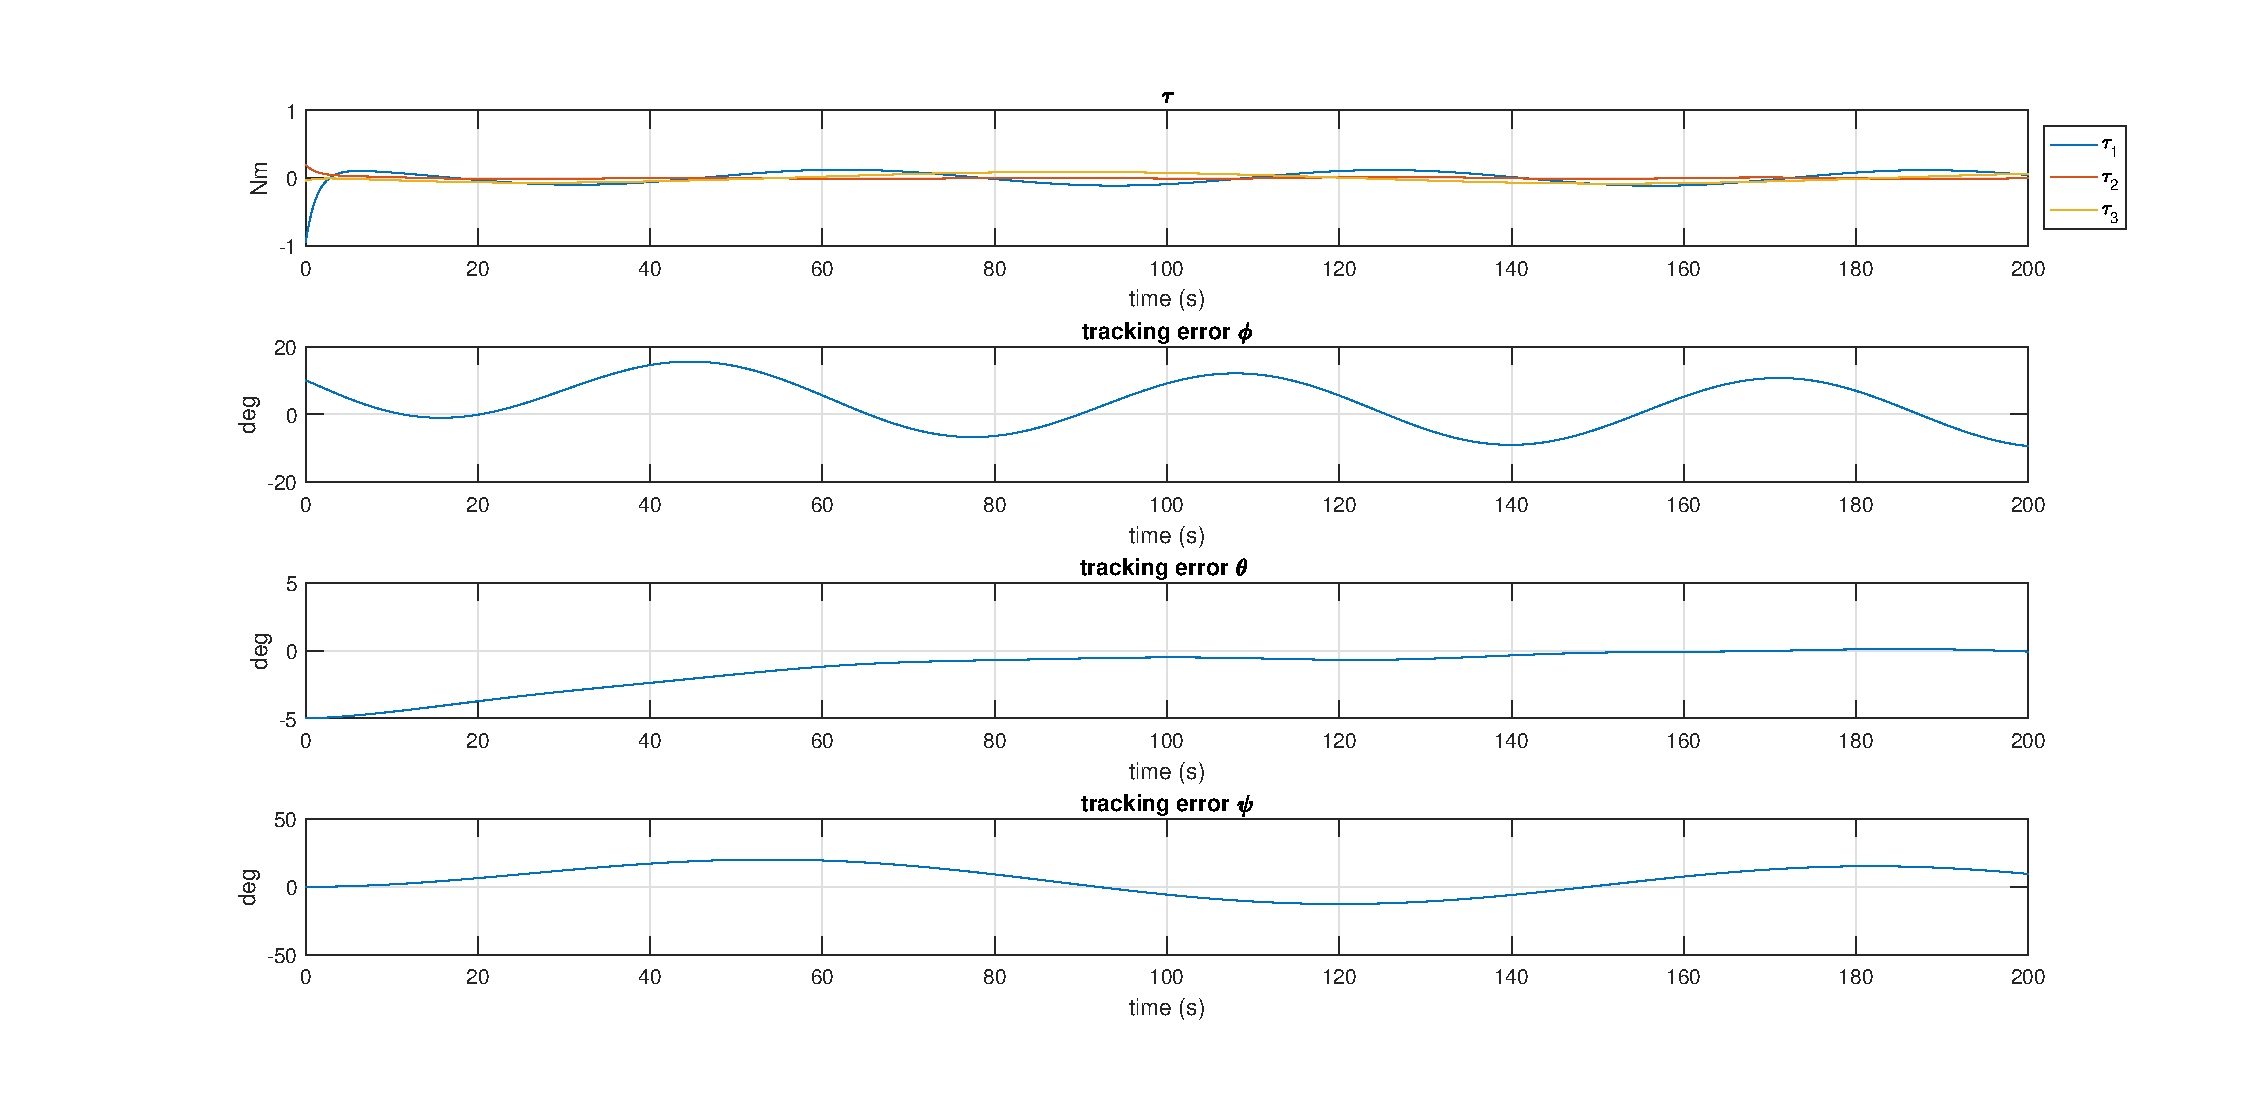
\includegraphics[width=1.00\textwidth]{figures/2_tau_track.eps}
	\caption{ $\boldsymbol{\tau}$, and the tracking errors of the output euler angles from the simulation in attitude2.m}
\label{fig:sim_attitude2_track}
\end{figure}


The Figures show that, with the exception of $\boldsymbol{\theta}$, the angles of the satellite are following a sinusoidal pattern as per their desired values. However, they are not in sync with the desired signal and the amplitude is far too low compared to their intended forms, resulting in relatively large sinusoidal tracking errors as can be seen in \Cref{fig:sim_attitude2_track}. A reason for this misbehaviour is the design of the controller. Our controller as of this problem may be sufficient for static point regulation. However, with frequently changing desired values as we have here, we receive poor results. The two parts of our states $\boldsymbol{\omega}$ and $\boldsymbol{\epsilon}$ are not decoupled, but this fact is lost on the controller as it lacks the nessesary connection between them. With the fact that, even though the angles of the satellite is set to move in a specific way, the desired value of $\boldsymbol{\omega}$ is still set to 0, makes for a contradiction in the controller where neither part is able to do as they are told. The exception is $\theta$ and $\omega_2$ who both have desired values of 0 and therefore does not obstruct each other. We would need to correct this in order to achieve satisfying control.

Increasing $k_p$ to 100 resulted in less error in the euler angles. This makes sense as a higher proportional part makes for a faster controller and puts more weight on the error in $\boldsymbol{\epsilon}$. 

It is also worth mentioning that the $\mathbf{K}$ matrix used for the controller was found using the linearized version of the system. This may also introduce errors.



\subsection*{Problem 1.6}
\addcontentsline{toc}{subsection}{Problem 1.6}

A modified attitude control law is:
\begin{equation}
    \boldsymbol{\tau} = -\mathbf{K}_d\tilde{\boldsymbol{\omega}} -k_p\tilde{\tilde{\boldsymbol{\epsilon}}}
    \label{eq:control_law_attitude3}
\end{equation}

with $\tilde{\boldsymbol{\omega}} = \boldsymbol{\omega} - \boldsymbol{\omega_d}$. Differentiating the desired attitude, $\Theta_d$, from the previous problem and calculating $\omega_d$ as

\begin{equation}
    \boldsymbol{\omega}_d = \mathbf{T}_{\boldsymbol{\Theta}_d}^{-1}(\boldsymbol{\Theta}_d)\dot{\boldsymbol{\Theta}_d}
    \label{eq:omega_d}
\end{equation}

To simulate the new closed-loop system, small changes was  done compared to the file {\color{blue} attitude2.m}. The new simulation file was named {\color{blue} attitude3.m}. To find $\mathbf{T}_{\boldsymbol{\Theta_d}}$ the \texttt{MATLAB} function \texttt{eulerang()} was used and set $k_p$ and $k_d$ to 10 and 300 respectively as before. The $\boldsymbol{\omega}_d$ was calculated from \eqref{eq:omega_d} and the new control law, equation \eqref{eq:control_law_attitude3}, was implemented   in the new simulation {\color{blue} attitude3.m}.

\subsubsection*{Simulation results}
\addcontentsline{toc}{subsubsection}{Simulation results}

We can see from \Cref{fig:sim_attitude3_euler} and \Cref{fig:sim_attitude3_omega} that the satellite is now able to follow the given reference signal for both angles and angle velocities. From \Cref{fig:sim_attitude3_track} we can see that though there still is an error in the $\phi$ and $\psi$ they are much smaller than previously. Now that $\boldsymbol{\omega}$ and $\boldsymbol{\epsilon}$ have corresponding desired values, they can both be satisfied by the same actions. The cooperation between the two parts of the state, which are in themselves related, is key to making a good controller. The linearization error discussed in the previous problem may still endure and the controller is not exactly the fastest in the galaxy, but all in all the attitude control is better than before.

\begin{figure}[!htb]
	\centering
	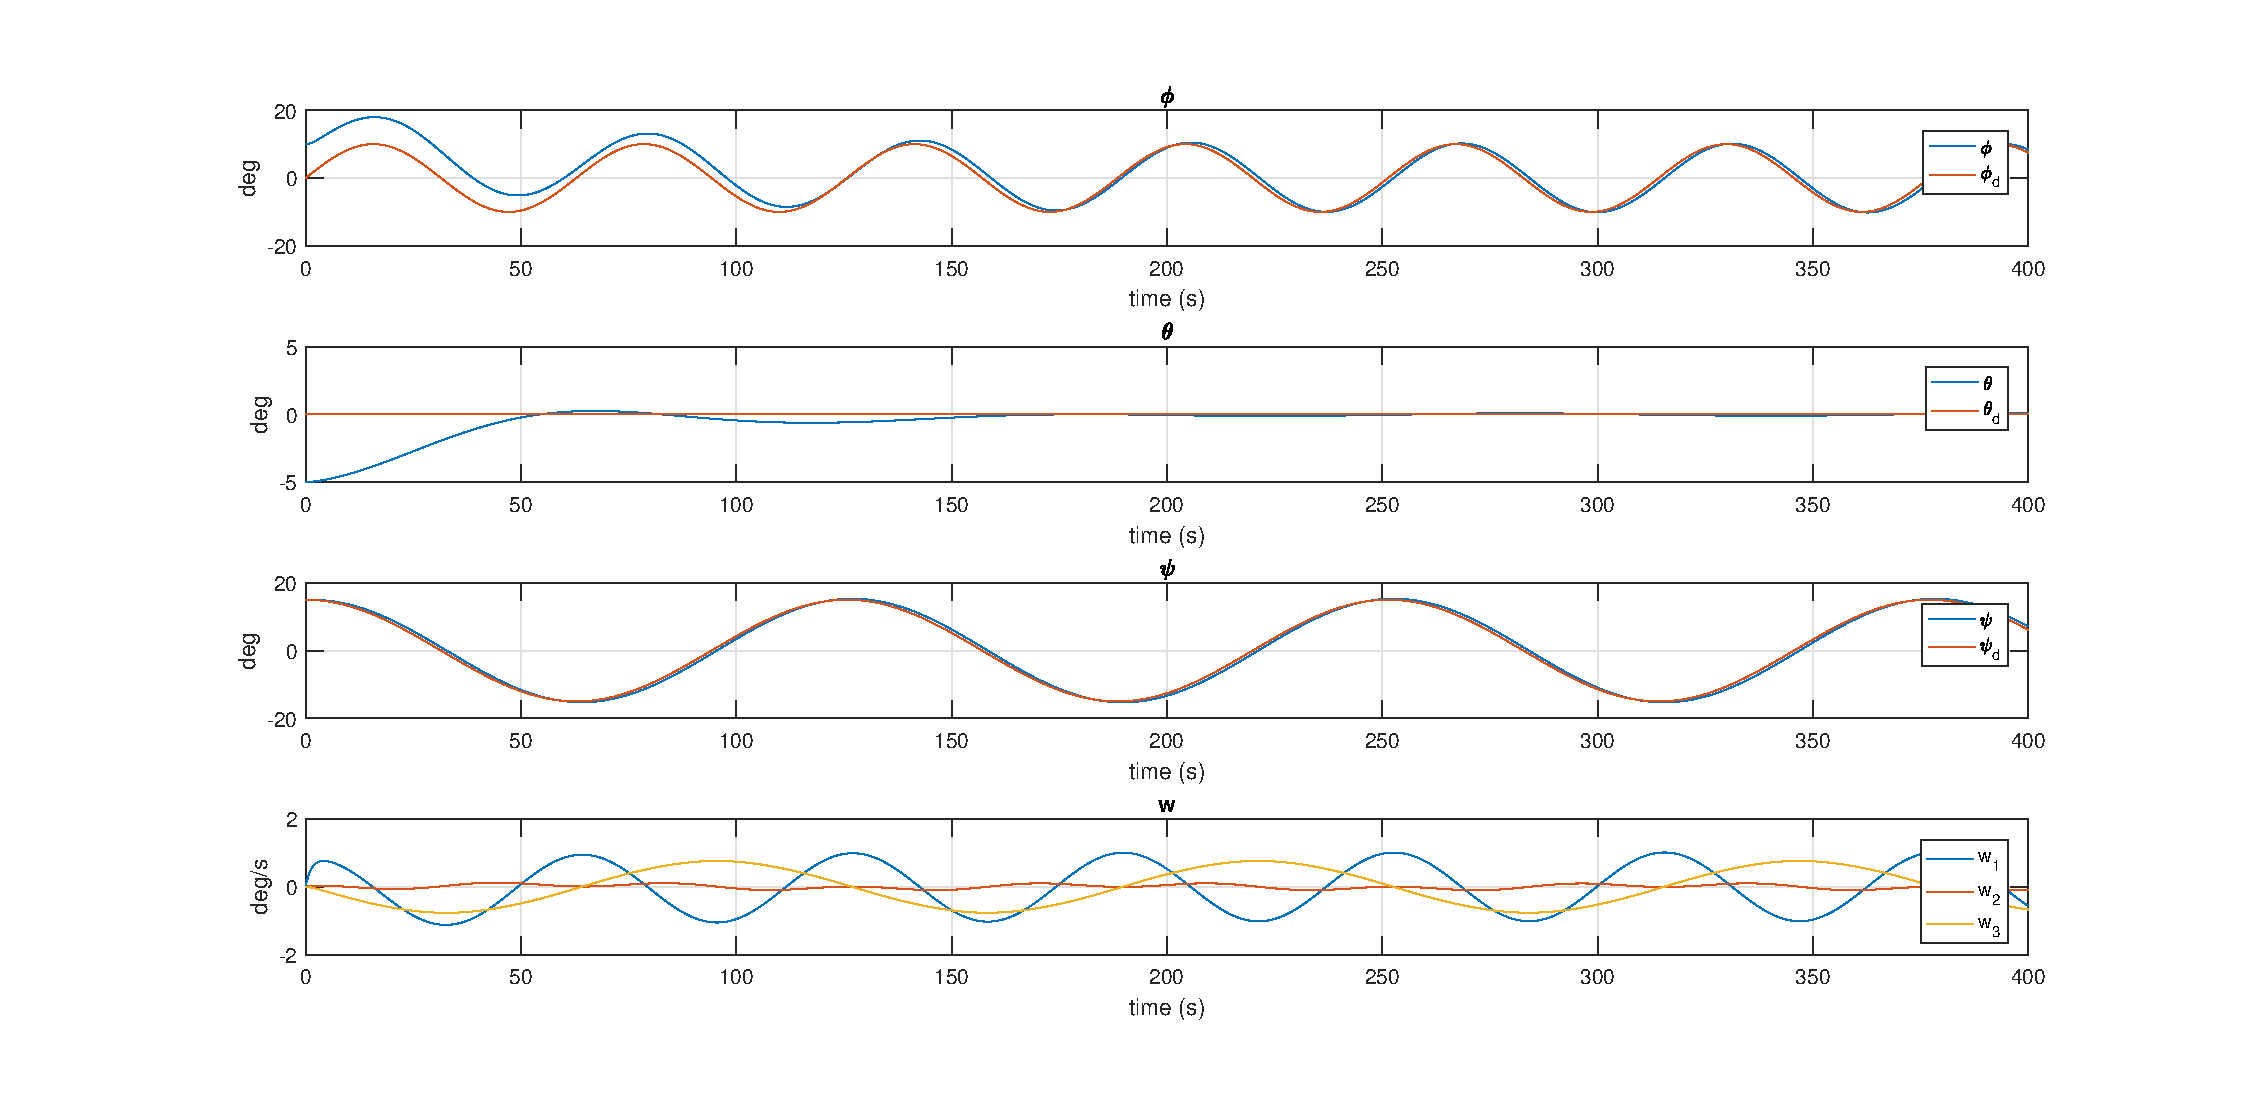
\includegraphics[width=1.00\textwidth]{figures/3_euler.eps}
	\caption{The resulting output euler angles with their corresponding desired values from the simulation in attitude3.}
\label{fig:sim_attitude3_euler}
\end{figure}

\begin{figure}[!htb]
	\centering
	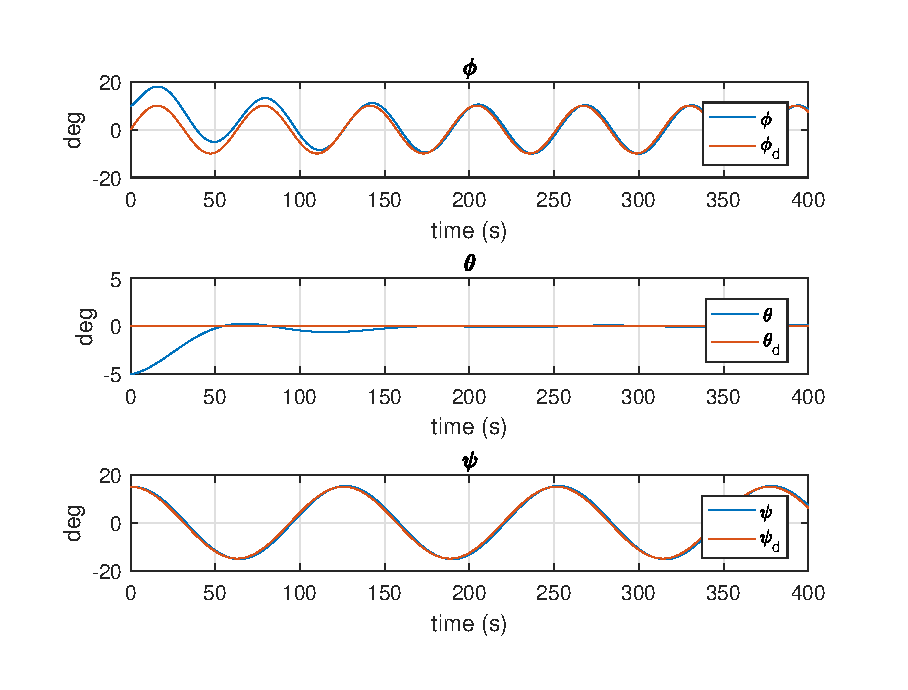
\includegraphics[width=1.00\textwidth]{figures/3_omega.eps}
	\caption{The resulting output $\boldsymbol{\omega}$ (denoted $\mathbf{w}$ in the plots) and the corresponding desired values from the simulation in attitude3.}
\label{fig:sim_attitude3_omega}
\end{figure}

\begin{figure}[!htb]
	\centering
	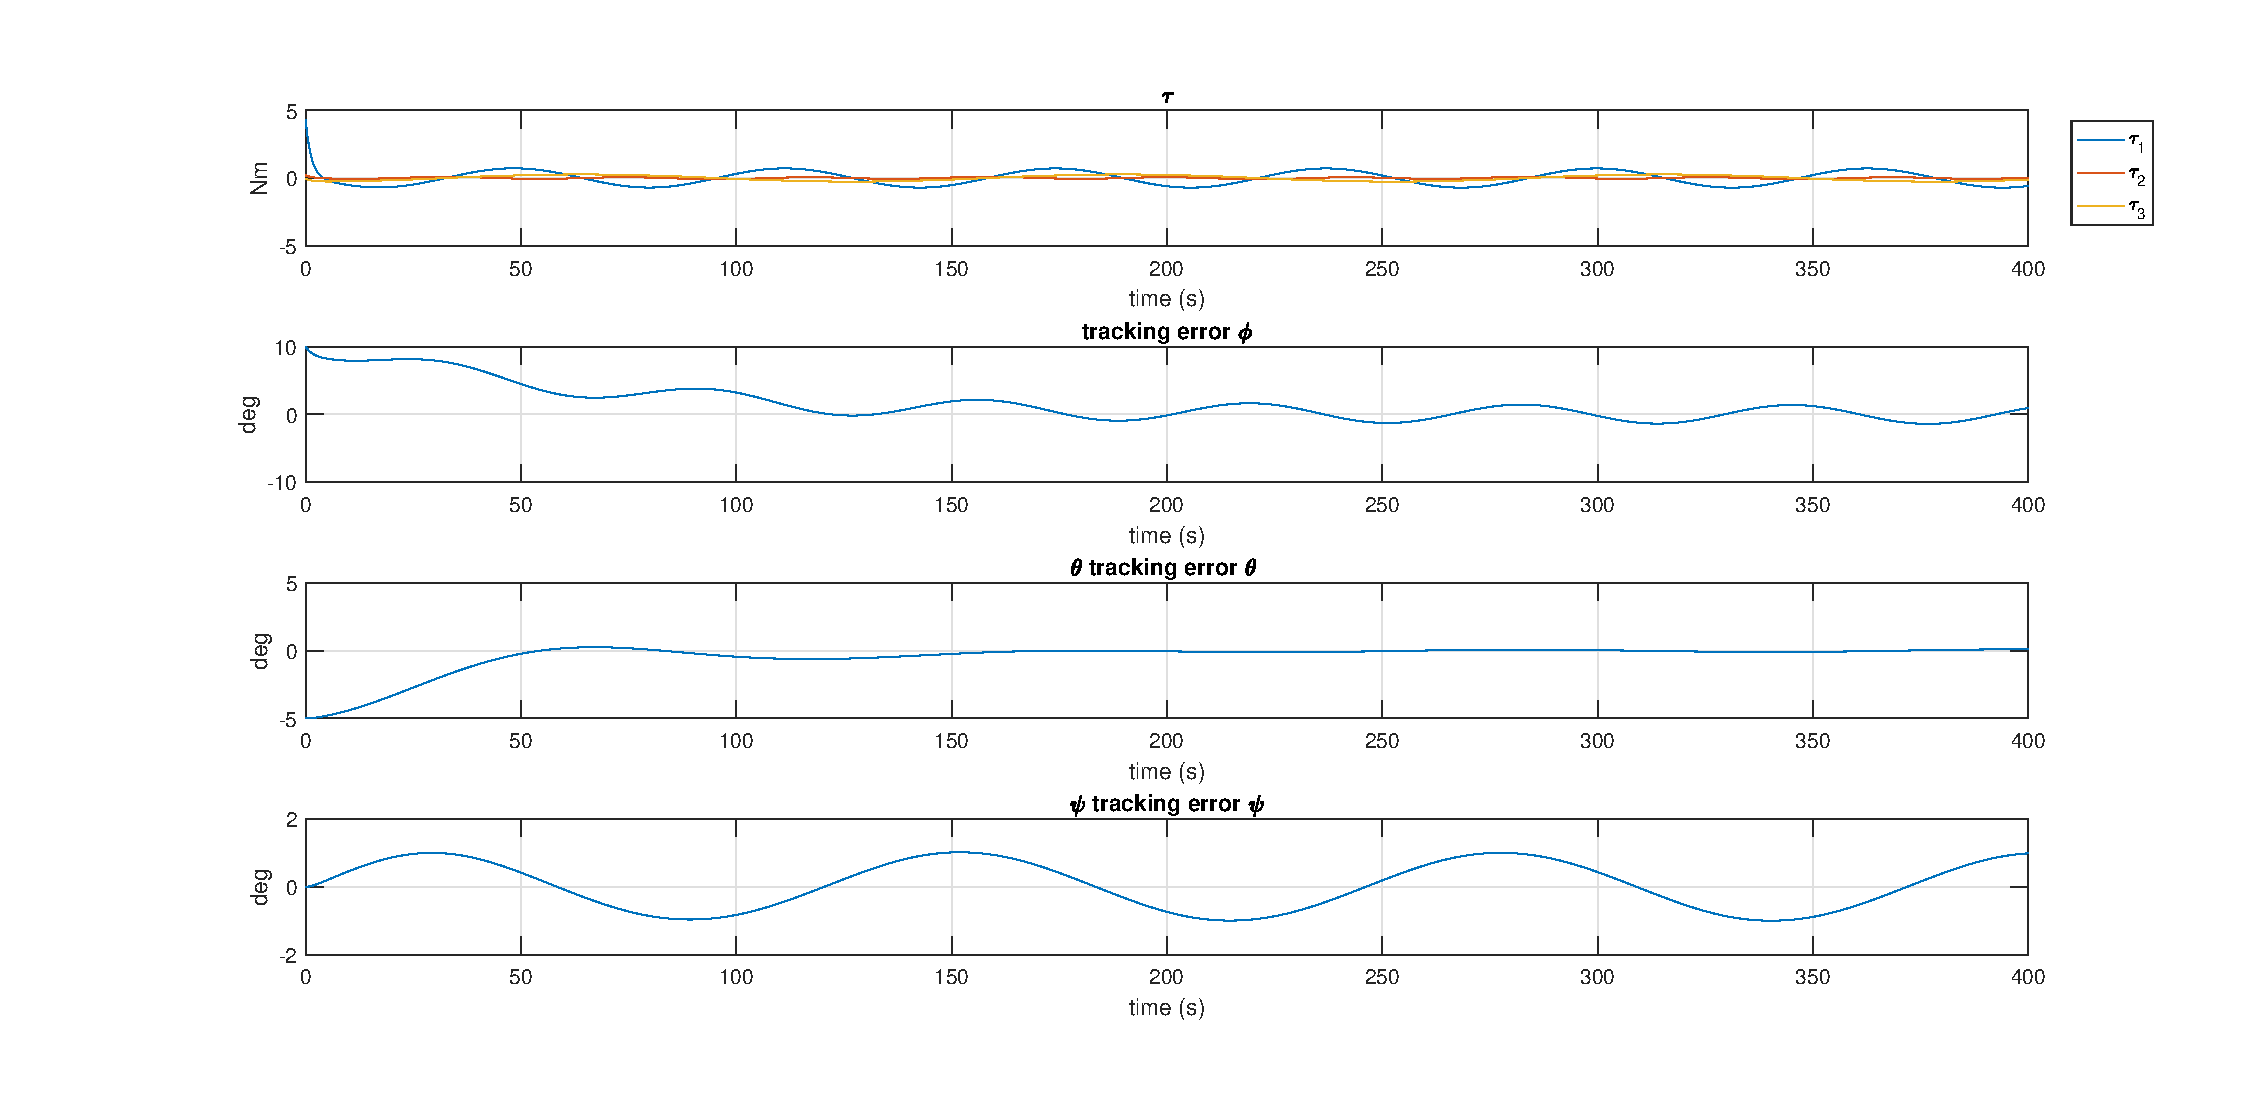
\includegraphics[width=1.00\textwidth]{figures/3_tau_track.eps}
	\caption{ $\boldsymbol{\tau}$, and the tracking errors of the output euler angles from the simulation in attitude3.}
\label{fig:sim_attitude3_track}
\end{figure}

\subsection*{Problem 1.7}
\addcontentsline{toc}{subsection}{Problem 1.7}

A Lyapunov function candidate (Fjellstad and Fossen, 1994) was given:

 \begin{equation}
	 V = \frac{1}{2} \tilde{\boldsymbol{\omega}}^{\top} \mathbf{I}_{CG}\tilde{\boldsymbol{\omega}} + 2 k_p (1-\tilde{\eta})
	 \label{eq:lyapunov}
 \end{equation}


Assuming $\boldsymbol{\omega_d }= \mathbf{0}$ and $\boldsymbol{\epsilon}_d$ and $\eta_d$ constants and the control law given by \eqref{eq:control_law_attitude2}, the Lyapunov function in equation \eqref{eq:lyapunov} is positive and radially unbounded. 

The reason for Vs positivity is that $\mathbf{I}_{CG}$ being an identity matrix with a positive number, $mr^2$, on its diagonal, is positive definite. So the first part of V is positive (when labeling 0 as a positive number). The second part, consisting of $2 k_p (1-\tilde{\eta})$, may only be negative if $\tilde{\eta} > 1$. This will never happen however, as $\tilde{\eta}$ is part of the unit quaternion $\tilde{q}$ making $|\tilde{\eta}| \leq 1$. Thus the second part of V will also be positive. The Lyapunov function is usually thought of as a representation of the energy in the system so the fact that it is never negative makes sense. 

The function is radially unbounded because as $\tilde{\boldsymbol{\omega}}\rightarrow \infty$ the first part of V does the same, $\frac{1}{2} \tilde{\boldsymbol{\omega}}^{\top} \mathbf{I}_{CG}\tilde{\boldsymbol{\omega}} \rightarrow \infty$. We already established that the second part of V, $2 k_p (1-\tilde{\eta})$ is positive, meaning that V as a whole is unbounded.

\subsubsection*{Calculating $\dot{V}$ }
\addcontentsline{toc}{subsubsection}{Calculating $\dot{V}$ }

To calculate $\dot{V}$ , $\tilde{\boldsymbol{\omega}} = \boldsymbol{\omega} - \boldsymbol{\omega}_d = \boldsymbol{\omega}$ was substituted into V before differentiating:

\begin{equation}
    \dot{V} = \boldsymbol{\omega}^\top\mathbf{I}_{CG}\dot{\boldsymbol{\omega}} + k_p\tilde{\boldsymbol{\epsilon}}^\top\boldsymbol{\omega} 
\end{equation}

Then, using \eqref{eq:EOM_omega_dot}, $\mathbf{I}_{CG}\dot{\boldsymbol{\omega}}$ was substituted giving this equation:

\begin{equation}
    \dot{V} = \boldsymbol{\omega}^\top(\boldsymbol{\tau} - \mathbf{S}(\mathbf{I}_{CG})\boldsymbol{\omega}) + k_p\tilde{\boldsymbol{\epsilon}}^\top \boldsymbol{\omega }
\end{equation}

Knowing $\boldsymbol{\omega}\mathbf{S}(\mathbf{I}_{CG})\boldsymbol{\omega} = 0$ and substituting $\boldsymbol{\tau}$ from the control law \eqref{eq:control_law_attitude2} in the equation, we are left with

\begin{equation}
    \dot{V} = \boldsymbol{\omega}^\top( k_d \boldsymbol{\omega} - k_p\tilde{\boldsymbol{\epsilon}}) + k_p\tilde{\boldsymbol{\epsilon}}^\top\boldsymbol{\omega} = -k_d\boldsymbol{\omega}^\top\boldsymbol{\omega}
\end{equation}


\subsubsection*{Convergence}
\addcontentsline{toc}{subsubsection}{Convergence of omega  to zero }

Barbalat's lemma (A.1)\cite{Fossen2011}, tells us that our $\boldsymbol{\omega}$ will converge to zero if three conditions are satisfied: 

\begin{itemize}
    \item $V \geq 0$
    \item $\dot{V} \leq 0$
    \item $\dot{V}$ is uniformly continuous
\end{itemize}

We already proved the first one when we proved V is positive. For the second condition we can easily see that $\dot{V}$ as a negative quadratic function, due to $\boldsymbol{\omega}^\top\boldsymbol{\omega} \geq 0$ and $k_d \geq 0$ a constant, must be $\leq 0$.

To prove $\dot{V}$ is uniformally continuous, we can take a look at $\ddot{V} = -2k_d\boldsymbol{\omega}^\top\dot{\boldsymbol{\omega}}$ and prove it to be bounded. We can assume the $\boldsymbol{\omega}$, and thereby V, does not begin at $\infty$ and we know $\dot{V}$ is negative, meaning V is always sinking. However V will always be positive, meaning it must stop at 0. Thus $\boldsymbol{\omega}$ will never increase beyond it's initial value. Knowing we are in physical system, it is reasonable to assume $\boldsymbol{\omega}$ is continuous, thus $\dot{\boldsymbol{\omega}}$ cannot go towards $\infty$. With neither $\boldsymbol{\omega} \rightarrow \pm\infty$ nor $\dot{\boldsymbol{\omega}} \pm\rightarrow \infty$, $\ddot{V} = -2k_d\boldsymbol{\omega}^\top\dot{\boldsymbol{\omega}}$ is bounded. Meaning $\dot{V}$ is uniformly continuous and Barbalat is satisfied. $\boldsymbol{\omega}$ will converge to zero. 

According to the curriculum book\cite{Fossen2011}, Barbalat's lemma only guarantees global convergence, meaning our convergence to the equilibrium point is indeed global.

\subsubsection*{Asymptotic stability}
\addcontentsline{toc}{subsubsection}{Asymptotic stability }

The system is a non-autonomous system so to check stability  LaSalle-Yoshizawa's teorem may be used. Three conditions must be satisfied in LaSalle-Yoshizawa's theorem (A.4)\cite{Fossen2011}

\begin{itemize}
    \item $V > 0$ and  $V(0) = 0$
    \item $\dot{V} \leq 0$
    \item V is radially unbounded
\end{itemize}

We have already proved the last two conditions earlier in this exercise. As for the first one, we have proved that V is always positive, i.e. $V \geq 0$. We also know $\mathbf{I}_{CG} > 0$, or positive definite. This means the first part of V is only equal to zero when $\boldsymbol{\omega} = 0$. As for the second part, we know $\eta$ to be a function of $\boldsymbol{\epsilon}$, specifically $\eta = \sqrt{1 - \boldsymbol{\epsilon}^\top\boldsymbol{\epsilon}}$. The second part is only 0 when $\eta = 1$ which only happens when $\boldsymbol{\epsilon} = 0$, meaning $V = 0$ only when it's input $\mathbf{x}$ is zero, otherwise $V > 0$. 


Why do we not get stuck? $\dot{V} = -k_d\boldsymbol{\omega}^\top\boldsymbol{\omega} \leq 0$, as already stated, and $V = 0$ only when $\boldsymbol{\omega} = 0$. This does however not mean $\dot{\boldsymbol{\omega}} = 0$. Using \eqref{eq:EOM_omega_dot} and inserting $\boldsymbol{\omega} = 0$ and $\boldsymbol{\tau}$ into the equation we get

\begin{equation}
    \dot{\boldsymbol{\omega}} = \mathbf{I}_{CG}^{-1}k_p\tilde{\boldsymbol{\epsilon}} \neq 0
\end{equation}

Since $\dot{\boldsymbol{\omega}} \neq 0$ unless $\tilde{\boldsymbol{\epsilon}} = 0$ we will not get stuck. We will continue until we have reached our desired value.

So LaSalle-Yoshizawa's teorem suggests we have UGAS. However, we are working with unit quaternions which, depending on $\eta$ may have more than one solution as $\eta$ may be positive or negative, making the question of global stability more complicated. This assignment have defined $\eta$ as positive only leaving only one singular solution, but the simulation has not. It is possible to add extra complexity, to the controller so that it will only allow for/choose the positive $\eta$s, thus assuring global stability. 


\subsection*{Problem 1.8}

In this assignment we have been using unit quaternions which have the advantage of being defined in the whole space. This is unlike euler angles which has singularities at $\pm 90^\circ$ in pitch meaning one will have local stability at best. The singularity of the euler angle is usually not a problem when controlling boats at sea, seeing how they won't reach this angle anyway (and if they do, it is already too late to save them). Considering this assignment is concerned with controlling a satellite in space however, reaching a pitch of $\pm 90^\circ$ is not that unlikely and thus, must be accounted for. Unit quaternions is then a good choice.

Sadly, as all things in life, the unit quaternions also have drawbacks. One of them being the fact that they are 4-dimensional vectors used to describe a 3-dimensional space. This causes them not to be unique as two quaternions may represent the same thing yet have different sings of $\eta$ as mentioned in the previous problem. This problem is absent from euler angle representation. Another drawback worth mentioning is the fact that, while we are used to describe the world using a 3-dimentional euler angles or similar representations, quaternions are less intuitive for most people.

 

